% !TeX spellcheck = ru_RU
% !TEX root=../main.tex

\begin{lecture}[Модели коллоидных растворов]
    Солюбилизация --- процесс самопроизвольного и обратимого проникновения в ядро мицеллы гидрофобных веществ.
    \begin{wrapfigure}[5]{r}{0.3\linewidth}
        \centering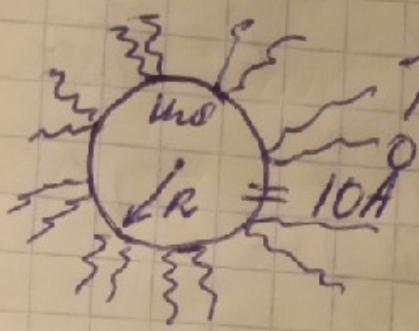
\includegraphics[width=\linewidth]{lecture_08/micella}
        \label{fig:micella}
        \caption{Модель мицеллы}
    \end{wrapfigure}
	\begin{align*}
		&R / _\text{HH} = 0.175 W_0 + 1.5 \\
		&w_0 < 20 \\
		R &= 33 \text{\,\AA~(н-гексан)} \\
		  &= 37 \text{\,\AA~(н-октан)}
	\end{align*}
	\begin{center}При $ R = 30\, \text{\AA} ~~ \eta \sim 10^2\, \text{cP} $.\end{center}
	
	\begin{lecSection}[Треугольник Гиббса]
		\begin{wrapfigure}[5]{r}{0.3\linewidth}
			\centering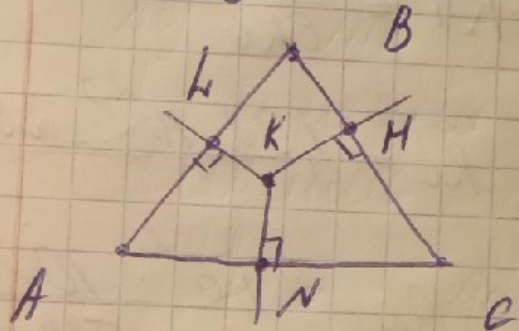
\includegraphics[width=\linewidth]{lecture_08/triangle_gibbs}
			\label{fig:triangle_gibbs}
			\caption{Треугольник Гиббса}
		\end{wrapfigure}
		\begin{equation*}
			KL + KH + KN = \text{высоте}
		\end{equation*}
		Хотим определить состав в $ K $:
		\begin{center}\noindent\begin{gather*}
		A \rightarrow KH \\
		B \rightarrow KN \\
		C \rightarrow KL
		\end{gather*}\end{center}
	\end{lecSection}

	\begin{lecSection}[Треугольник Розебума]
		\begin{wrapfigure}[5]{r}{0.3\linewidth}
			\centering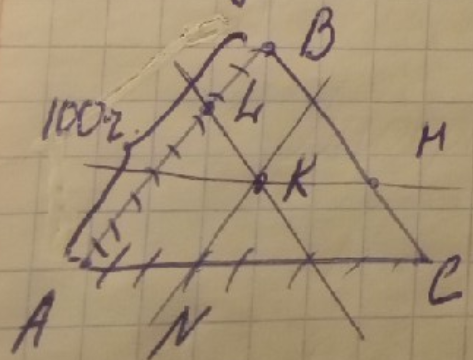
\includegraphics[width=\linewidth]{lecture_08/triangle_rozebum}
			\label{fig:triangle_rozebum}
		\end{wrapfigure}
	\begin{gather*}
		A \rightarrow KM \\
		B \rightarrow KN \\
		C \rightarrow KL
	\end{gather*}
	
	\centering\underline{\textbf{Пример}}:
	\begin{figure}[H]
		\centering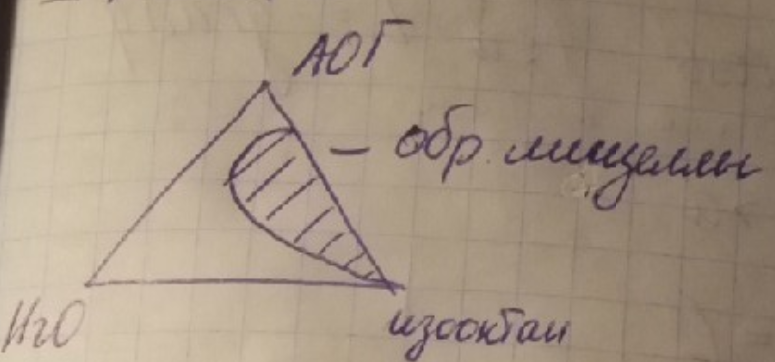
\includegraphics[width=0.7\linewidth]{lecture_08/triangle_example}
		\label{fig:triangle_example}
	\end{figure}
	\end{lecSection}
	
	% Костыль на wrapfigure от диполя
	\vspace{-1.3cm}
	\begin{lecSection}[Модель Онзагера]
		% Костыль на wrapfigure от диполя
		\vspace{-1cm}
		\begin{wrapfigure}[4]{r}{0.3\linewidth}
			\centering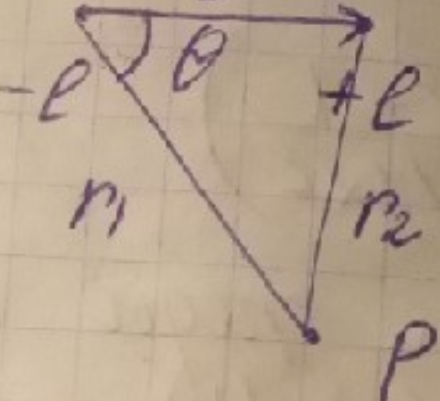
\includegraphics[width=\linewidth]{lecture_08/dipole}
			\label{fig:dipol}
			\caption{Меня все равно не увидят :)}
		\end{wrapfigure}
	
		\begin{gather*}
			m = e l \\
			\varphi_p = e \left( \dfrac{1}{r_2} - \dfrac{1}{r_1} \right) \\
			r^2 \simeq r_1 r_2 \\
			(r_1 - r_2) = l \cos \theta \\
			\varphi = \dfrac{m \cos \theta}{r^2}
		\end{gather*}
				\begin{wrapfigure}[4]{r}{0.4\linewidth}
			\centering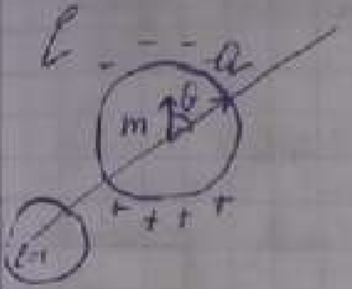
\includegraphics[width=\linewidth]{lecture_08/polar_sphere}
			\caption{
				\textit{Верху:} модель диполя; 
				\newline \textit{Внизу:} схема нашей задачи
			}
			\label{fig:polar_sphere}
		\end{wrapfigure}
		Рассмотрим полярную молекулу
	
		Мы хотим понять, как меняется энергия системы при растворении в ней диполей. Для этого нам понадобятся сведения из электродинамики, но перед этим напомним, что такое уравнение Лапласа:
		
		\begin{tabular}{cl}
			ур. Лапласа & $ \nabla^2 \varphi = 0 $ \\
			\multicolumn{2}{c}{$ \nabla^2 = \dfrac{\partial^2}{\partial x^2} + \dfrac{\partial^2}{\partial y^2} + \dfrac{\partial^2}{\partial z^2} $} \\
			Граничные условия: & 1) $ \varphi $ -- непрерывная \\
							  & 2) $ \left.\dfrac{\partial \varphi}{\partial r} \right|_{a \neq 0} = \varepsilon \left. \dfrac{\partial \varphi}{\partial r} \right|_{a \neq 0} $ \\
			\multicolumn{2}{c}{Решение ищется подстановкой:} \\
			\multicolumn{2}{c}{$ \varphi = \sum\limits_{n=0}^\infty \left( A_n r^n + \dfrac{B_n}{r^{n+1}} \right) Y (\theta, \varphi) $}
		\end{tabular}
		
		\begin{gather*}
			\begin{cases}
				\varphi = \dfrac{m \cos \theta}{r^2} - \underbrace{R r \cos \theta}_{ \text{поле отклика} }, ~~ r \leq a, ~~ \vec{E} = - \nabla \varphi \\
				\varphi = \dfrac{l \cos \theta}{l r^2}, ~~ r > a
			\end{cases}
		\end{gather*}
		\begin{center}\begin{tabular}{cl}
			1 гр. & $ \rightarrow ml - R l a^3 = C $ \\
			2 гр. & $ \rightarrow -\dfrac{2m}{a^3} - R = -\dfrac{2C}{a^3} $ \\
		\end{tabular}\end{center}
		% Костыль на wrapfigure от диполя
		\hspace{2cm}
		\begin{gather}
			\nonumber
			2m + R a^3 = 2 ml - 2Rl a^3 \\
			\boxed{ R = \dfrac{2m}{a^3} \left( \dfrac{\varepsilon - 1}{1 + 2l} \right) } \\
			\nonumber
			\text{--- электрическая реакция среды на диполь}
		\end{gather}
		Уменьшение энергии Гиббса при введении диполя составит: $ \Delta G = - m \vec{R} = - \dfrac{2 m^2}{a^3} \left( \dfrac{\varepsilon - 1}{1 + 2l} \right) $. Это уравнение справедливо для стационарного случая.
		
		При малых времена жизни диполей справедлива связь: $ \varepsilon = n^2 $
		\begin{equation}
			\Delta G = - \dfrac{2 m^2}{a^3} f( \varepsilon )
			\label{eq:deltaG_from_epsilon}
		\end{equation}
		
		Модель Дебая дает выражение для этой функции $ f( \varepsilon) = \dfrac{\varepsilon - 1}{ \varepsilon + 1} $
		
		\begin{lecSection}[Выборочная сольватация]
%			Костыль: убираю все в таблицу, чтобы избежать использования wrapfigure. Он и правда ужасен!
			\begin{tabular}{cc}
				Выборочная сольватация ($ B $ взаимодействует лучше, чем $ A $) $ \rightarrow $ & \multirow{3}{*}{
					\centering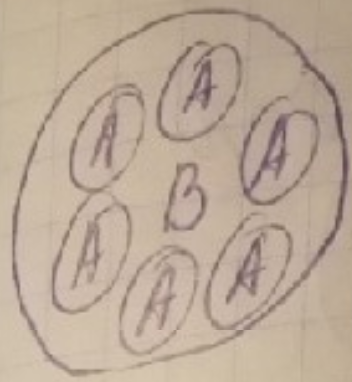
\includegraphics[width=0.3\linewidth]{lecture_08/selective_solvation}
				} \\
				$ < 10 \% $ об. &  \\
				ДНСО/бензол & \\
				(Для ДНСО $ \varepsilon = 60 $, бензол же неполярный растворитель) & \\
				соль + ДНСО $ \rightarrow $ бензол (соль растворена в бензоле) & \\
				\vspace{2cm}
			\end{tabular}
		\end{lecSection}
	
		\begin{lecSection}[Актуальная супрамолекулярная система]
			Кукурбитурилы (подоходят для транспортировки лекарств) -- один из примеров супрамолекулярных систем.
			\begin{figure}[H]
				\begin{minipage}[h]{0.48\linewidth}
					\centering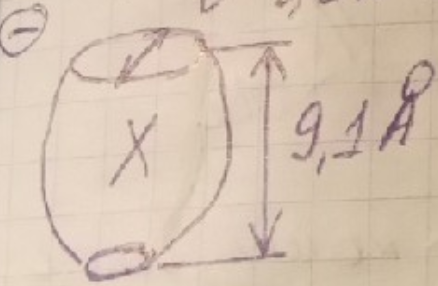
\includegraphics[width=\linewidth]{lecture_08/kukur_scheme}
					\caption{Схематическое изображение кукурбитурила}
				\end{minipage}
				\hfill
				\begin{minipage}[h]{0.48\linewidth}
					\centering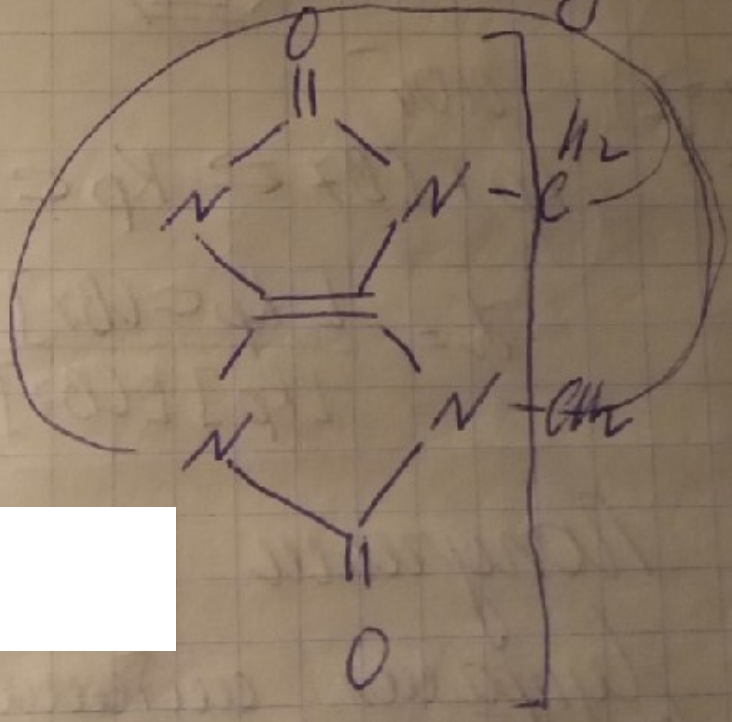
\includegraphics[width=0.8\linewidth]{lecture_08/kukur_border}
					\caption{Внешняя оболочка кукурбитурила}
				\end{minipage}
				\hfill
			\end{figure}
		
			Эти вещества образовывать комплексы, а значит, и могут защищать молекулу от внешней среды и наоборот. Это и делает данный класс веществ перспективными для производства лекарств.
		\end{lecSection}
	\end{lecSection}
	
\end{lecture}
